\section{Architecture Integration}

\subsection{Model Support}

\begin{table}[H]
\centering
\small
\begin{tabular}{lllll}
\toprule
\textbf{Model} & \textbf{Attention class} & \textbf{Nested?} & \textbf{RoPE?} & \textbf{GQA?} \\
\midrule
DistilBERT & \texttt{MultiHeadSelfAttention} & No & No & No \\
RoBERTa & \texttt{BertSelfAttention} (nested) & Yes & No & No \\
GPT-2 & \texttt{GPT2Attention} (Conv1D) & No & No & No \\
Qwen3.5 & \texttt{Qwen3Attention} & No & Yes & Yes \\
\bottomrule
\end{tabular}
\end{table}

\subsection{Weight Transfer}

We copy base weights from the pretrained attention via \texttt{copy\_weights}, which 
handles four patterns:

\subsubsection{Pattern 1: GPT-2 Conv1D}

\begin{lstlisting}
c\_w = src.c\_attn.weight.t()  # Conv1D stores (in, out); transpose
q\_w, k\_w, v\_w = c\_w.chunk(3, dim=0)
\end{lstlisting}

\subsubsection{Pattern 2: RoBERTa Nested}

\begin{lstlisting}
if hasattr(src, "self") and hasattr(src, "output"):
    self.is\_nested\_encoder = True
    q\_w = src.self.query.weight
    k\_w = src.self.key.weight
    v\_w = src.self.value.weight
    o\_w = src.output.dense.weight
\end{lstlisting}

\subsubsection{Pattern 3: Qwen/LLaMA (GQA)}

\begin{lstlisting}
q\_w = src.q\_proj.weight  # (H d\_h, d)
k\_w = src.k\_proj.weight  # (H\_kv d\_h, d)
v\_w = src.v\_proj.weight
o\_w = src.o\_proj.weight
\end{lstlisting}

\subsubsection{Pattern 4: DistilBERT}

\begin{lstlisting}
q\_w = src.q\_lin.weight
k\_w = src.k\_lin.weight
v\_w = src.v\_lin.weight
o\_w = src.out\_lin.weight
\end{lstlisting}

\subsubsection{Pattern 5: UniversalAdapter Fallback}

If none of the above patterns match, we use \texttt{UniversalAdapter.get\_weight\_bias}.

\subsection{Nested Encoder Bypass}

For RoBERTa, we set \texttt{is\_nested\_encoder = True}, meaning our \texttt{forward} returns 
raw context and the outer \texttt{BertSelfOutput.dense} applies the output projection.

\subsection{Causal Mask Construction}

The most delicate part. For decoders:

\begin{lstlisting}
q\_pos = torch.arange(L).view(1, 1, L, 1)
k\_orig\_pos = top\_idx.unsqueeze(1).unsqueeze(2)  # (B, 1, 1, k)
causal\_mask = (k\_orig\_pos \textgreater{} q\_pos)
scores = scores.masked\_fill(causal\_mask, float("-inf"))
\end{lstlisting}

\textbf{Why this is correct.} Even though compressed keys are indexed $0..k-1$, 
their original positions \texttt{top\_idx} are what matters. Query at position $i$ 
can attend only to keys whose original position is $\leq i$.

\textbf{Verification.} We check that output at position $i$ depends only on 
inputs $\leq i$ by computing gradients.

\subsection{Handling Padding}

Padding tokens are masked out of the score:

\begin{lstlisting}
total\_importance = total\_importance.masked\_fill(mask == 0, -10000.0)
\end{lstlisting}

After selection, the compressed mask is gathered:

\begin{lstlisting}
comp\_mask = torch.gather(mask, 1, top\_indices)
\end{lstlisting}

\subsection{Injection Algorithm}

\textbf{Algorithm 2:} Inject TCA into a model
\begin{lstlisting}
Input:  model M, compression\_ratio  
Output: M with attention replaced

1: for   in transformer\_layers(M) do
2:     src $\leftarrow$ get\_attention( )
3:     new $\leftarrow$ TokenCompressedAttention(config,  , pretrained\_attn=src)
4:     replace( , new)
5: end for
6: return M
\end{lstlisting}

\subsection{The `score\_net` Module}

\begin{lstlisting}
self.score\_net = nn.Sequential(
    nn.Linear(self.dim, 64),
    nn.GELU(),
    nn.Linear(64, 1),
)
\end{lstlisting}

Total parameters: \texttt{dim \textit{ 64 + 64 + 64 + 1 = 65}dim + 65}. For $d = 768$: 
\textbf{49,985 parameters} per layer.

\subsection{Failure Modes and Fallbacks}

\begin{table}[H]
\centering
\small
\begin{tabular}{lll}
\toprule
\textbf{Failure} & \textbf{Detection} & \textbf{Response} \\
\midrule
Weight extraction fails & Exception in copy\_weights & Raise RuntimeError \\
Score net NaN & \texttt{torch.isnan} on scores & Fallback to norm-only \\
All tokens masked & \texttt{k\_keep = 0} & Force k\_keep = 1 \\
Short sequence & $L \leq 2$ & Skip compression \\
Causal leak & Grad check & Not observed \\
\bottomrule
\end{tabular}
\end{table}

\subsection{Registry}

\begin{lstlisting}
@ATTENTION\_REGISTRY.register("token\_compressed")
@ATTENTION\_REGISTRY.register("token\_compressed\_attention")
@ATTENTION\_REGISTRY.register("token\_compressed\_module")
class TokenCompressedAttention(BaseAttention):
    ...
\end{lstlisting}
\begin{lstlisting}

---
\end{lstlisting}

\begin{figure}[H]
\centering
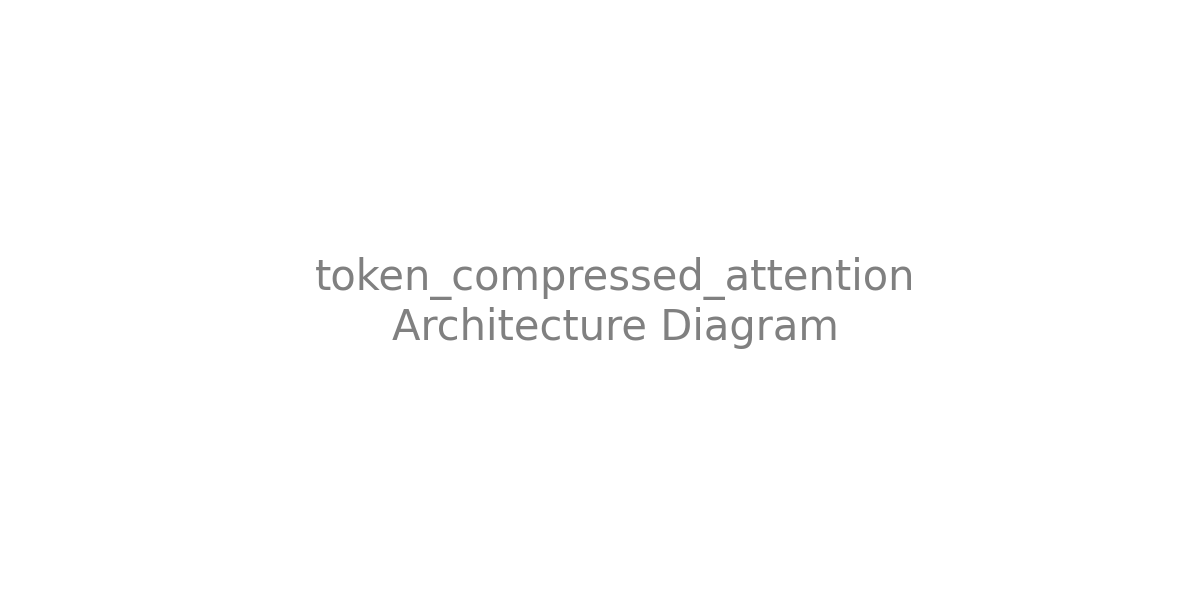
\includegraphics[width=\linewidth]{figures/architecture.png}
\caption{High-level architectural diagram of token\_compressed\_attention.}
\label{fig:arch_token-compressed-attention}
\end{figure}

